\chapter{Experimental Results} % (fold)
\label{cha:experiments}

This chapter presents the experimental work completed to validate the actuator dynamics and motion control framework. The hardware platform used for experimental validation is presented in Section~\ref{sec:physical_hardware}. This includes the mechanical implementation of the bipedal robot design and the control electronics used to control the robot. 

The simulations used to demonstrate the proposed 3D FPE walking control strategy in the previous section accounted for link side dynamics only. Section~\ref{sec:actuator_model} describes the modifications to account for the actuator dynamics. This modification to the simulations enables a single controller designed in Simulink to target either the simulation environment or the physical hardware using the HIL architecture discussed in Section~\ref{sec:hil_architecture}. The experimental validation for a single actuator and the proposed motion control framework are presented in Sections \ref{sec:1dof_validation} and \ref{sec:motion_control_validation}, respectively. 

\section{Physical Hardware} % (fold)
\label{sec:physical_hardware}
The electromechanical design presented in Chapter~\ref{cha:design} was realized to develop the 14 DOF bipedal robot. The assembled 7 DOF leg of the biped is shown in Figure~\ref{fig:bipedleg}. The mechanical implementation was derived directly from the revised CAD models. The control electronics were developed by an industry partner, Quanser Inc. This section presents the realization of the physical hardware platform used for experimental validation. 

\begin{figure}[!h]
	\centering
    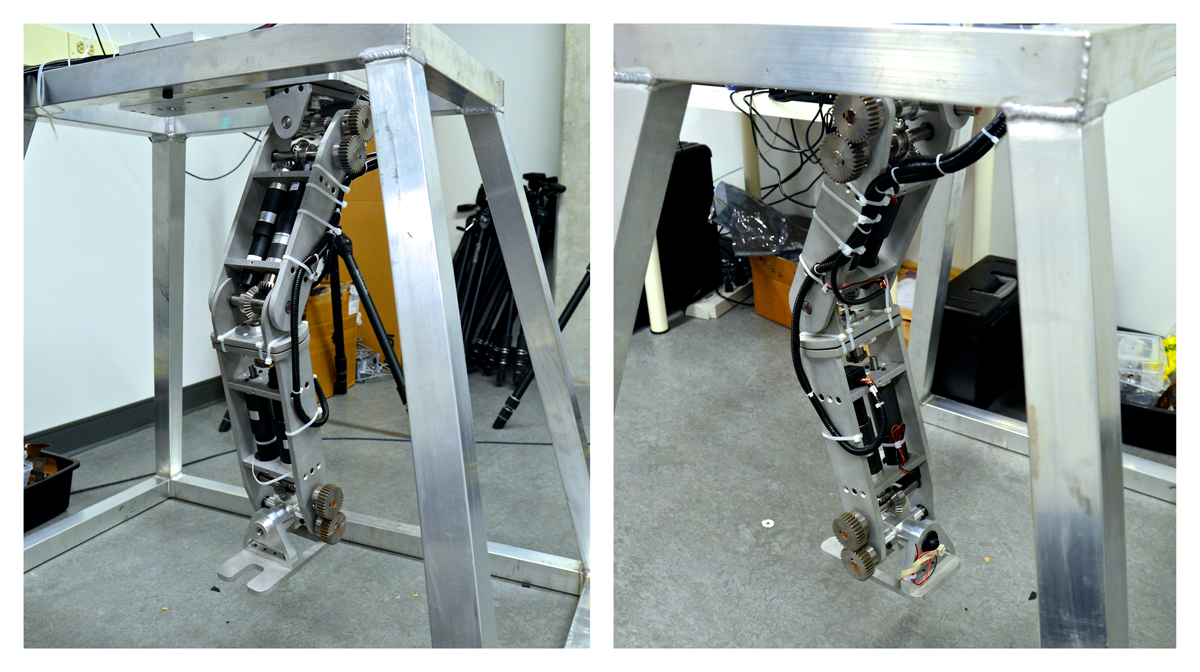
\includegraphics[scale=0.39]{fig/hardware/bipedleg.png} 
  	\caption{The 7 DOF leg built for the bipedal robot based on the electromechanical design in Chapter~\ref{cha:design}.}
	\label{fig:bipedleg}
\end{figure}

\subsection{Mechanical Implementation} % (fold)
\label{sub:mechanical_implementation}

The final mechanical design of the bipedal robot was developed on campus at the University of Waterloo. The on-site engineering machine shop manufactured the mechanical chassis components from the final CAD drawings (shown in Appendix~\ref{app:bipedcad}). The selected DC motors and gearhead combinations were sourced from a motor manufacturer. The drivetrain components (i.e. bearings, shafts, gears) used to relocate the output gearhead shaft from each joint axis were also sourced from a hardware vendor. The author of this thesis completed the mechanical assembly using the CAD model as a reference. The assembled joints and links of the bipedal robot leg are shown in more detail in Figure~\ref{fig:bipedcloseup}.

\begin{figure}[!h]
	\centering
    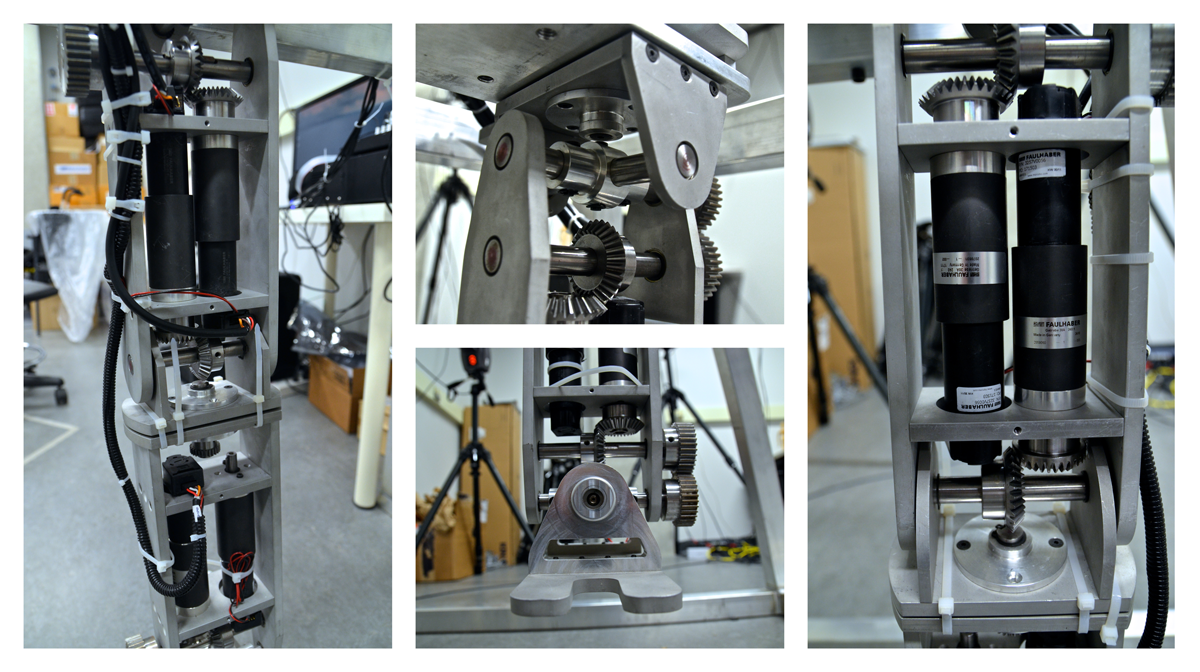
\includegraphics[scale=0.38]{fig/hardware/bipedcloseup.png} 
  	\caption{Close up pictures of various joints and linkages in the mechanical implementation of the bipedal robot design.}
	\label{fig:bipedcloseup}
\end{figure}

The mechanical chassis was composed primarily out of Aluminum 5052 and created using Computer Numerical-Controlled (CNC) machine tools directly from the CAD files. This enabled repeatable and accurate positioning of mechanical features in the chassis components (i.e. for the separation of holes for gearing components to mesh well). CNC machine tools also facilitated the production since some chassis components (i.e. motor mounts) were used multiple times in the design of each leg. The advantage here was that once the machine was setup to produce the first component, the remaining copies could be produced faster using the same setup. 

One of the key challenges in the assembled leg was the use of bevel gears for perpendicular mechanical coupling. It was difficult to position the gear axis with enough accuracy to achieve perfect clearance between mating components. As a result, some of the joints which use this design approach to shift the weight distribution suffer from backlash (or ``joint play''). In the current design, this is particularly evident for the knee joint, where one of the stock gearing components had to be modified due to fitment issues. 

In addition to developing the bipedal robot, a supporting frame was also designed for fixed and walking experiments (CAD drawings available in Appendix~\ref{app:framecad}). In the fixed configuration, the biped's torso is mounted directly to the frame. This provides sufficient ground clearance for the legs to remain suspended in the air. This removes the $n = 6$ unactuated DOF from the floating base but provides an experimental platform for testing basic control strategies (i.e. controlling swing foot motion). The walking configuration was designed to provide sufficient clearance for the biped to be mobile, while using a tether to provide support in case of a fall. 
% subsubsection mechanical_implementation (end)

\subsection{Control Implementation} % (fold)
\label{sub:control_implementation}

\begin{figure}[!b]
	\centering
    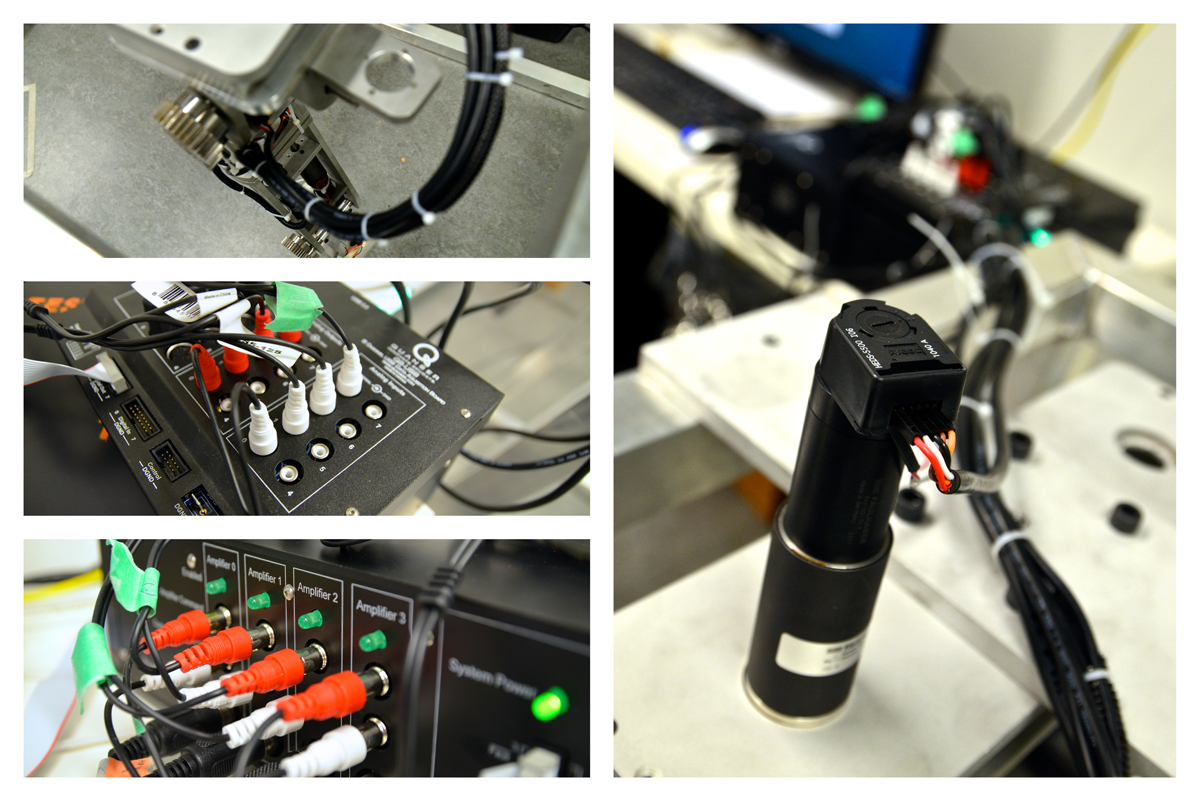
\includegraphics[scale=0.39]{fig/hardware/bipedwired.png} 
  	\caption{Electronics and wiring used to interface control loops running in Simulink to the physical hardware.}
	\label{fig:bipedwired}
\end{figure}

The electronics used for controlling the bipedal robot were developed by an industry partner. Quanser Inc developed custom motor controllers and drivers for the current requirements derived from torque estimates in dynamic simulations. Each joint in the bipedal robot has a (dedicated) local motor controller and driver unit. A control system model developed in Matlab/Simulink using Quanser's QUARC toolbox communicates with the electronics hardware through a serial interface (USB). Quanser's system enables hardware-in-the-loop (HIL) experiments with the physical bipedal robot (described further in Section~\ref{sec:hil_architecture}).    

Unfortunately, the electronics hardware developed by Quanser was not ready in time for experimental validation. Since it is a custom solution, further development was required before it could be used to control the complete 14 DOF bipedal robot. Quanser provided the author with control electronics from their existing product offerings in the interim to complete \emph{some} experimental validation on the physical robot. The general idea is that the HIL experiment models developed to target the interim solution could easily be switched to target the custom solution once it is ready. The interim solution is constrained to 7 channels. A single 7 DOF leg shown in Figure~\ref{fig:bipedwired} was wired to these channels for the experimental validation in this chapter. 

% subsubsection electronics_implementation (end)

% section physical_hardware (end)

\section{Actuator Model} % (fold)
\label{sec:actuator_model}
PD control is applied for each joint in order to track the desired trajectory generated by higher levels of control (Section~\ref{sub:control_strategy}). The control signal $u$ produced at each joint $k$ is provided by (where $k = 1 \ldots n$ is the $k$-th joint of the $n$-DOF system): 

\begin{equation}
	{u_k} = {K_P}({q_{d_k}} - {q_k}) - {K_D}{\dot q_k}
	\label{eq:pdcontrollaw}
\end{equation} 

Where ${q_{d_k}}$ and ${q_k}$ are the desired and actual angles and ${\dot q_k}$ is the velocity of the $k$-th joint. Constants ${K_P}$ and ${K_D}$ are the porportional and derivative gains of the controller, respectively. In the ideal case, the control signal ${u_k}$ would simply be applied to torque ${\tau _k}$ of each joint to form $\vtau = \left[\tau _1 \ldots \tau _k \right]$ shown on the right hand side of (\ref{eq:eom1}). However, the actuator dynamics of DC motors used in the development of the 14 DOF bipedal robot must be considered. The motors selected in Section~\ref{sub:final_configurations} are controlled by a voltage control signal $v_{m}$. A second order system is used to model the actuator dynamics and relate the applied torque to the motor voltage $v _m$ \cite{Spong2008}: 

\begin{equation}
	{J_m}{\ddot \Theta _m} + \left( {{B_m} + \frac{{{k_b}{k_m}}}{{{r_a}}}} \right)\dot \Theta _m  = {\tau _m} - \frac{{{\tau _l}}}{{{g_r}}}
	\label{eq:actdyn1}
\end{equation}

Where $\Theta _m$ is the rotor angle, $J_m$ is the motor inertia, $B_m$ is the motor damping, $k_b$ is the back emf or voltage constant, $k_m$ is the torque constant, $r_a$ is the armature resistance and $g_r$ is the gear reduction ratio. The motor torque $\tau _m$ is related to the (link side) load torque $\tau _l$ through the gearing ratio $g_r$. Since the output side of the gearhead is coupled directly to the link, the motor angles are related to the joint angles by: 

\begin{equation}
	{\Theta _{m_k}} = {g _{r_k}} {q _k}
	\label{eq:actdyn2} 
\end{equation}

Similarly, the joint torques in $\vtau$ (\ref{eq:eom1}) are related to the actuator load torques by: 

\begin{equation}
	{\tau _{m_k}} = {\frac{\tau _{k}}{g _{r_k}}} 
	\label{eq:actdyn3}
\end{equation}

Furthermore, the motor torque is related to the applied voltage through the following relationship: 

\begin{equation}
	{\tau _{m_k}} = {k_m} {i_a} = \left( {\frac{{{k_m}}}{{{r_a}}}} \right){v _{m_k}}
	\label{eq:actdyn4}
\end{equation}


Where $i_a$ is the current through the armature wiring. Substituting equations (\ref{eq:actdyn2} - \ref{eq:actdyn4}) back into (\ref{eq:actdyn1}) yields the complete relationship between the $k$-th joint angle, link side torque and the applied motor voltage:

\begin{equation}
	g_r^2{J_m}{\ddot q_k} + g_r^2\left( {{B_m} + \frac{{{k_b}{k_m}}}{{{r_a}}}} \right){\dot q_k} = g_r^{}\left( {\frac{{{k_m}}}{{{r_a}}}} \right){v_k} - {\tau _k}
	\label{eq:actdyn5}
\end{equation}

Note that the drivetrain constants specific to the $k$-th joint are used (i.e. ${J _{m_k}}$, ${B _{m_k}}$, $g _{r_k}$, etc.) in this equation (\ref{eq:actdyn5}). 

\subsection{Independent Joint Control} % (fold)
\label{sub:independent_joint_control}

% subsection independent_joint_control (end)

Using independent joint control \cite{Sciavicco2001}, each joint $k$ of the system is decoupled from the rest of the system and controlled individually. The control signal for each joint is computed directly from its own reference trajectory, position and velocity. This approach does not account for the coupled dynamics of the overall system described by (\ref{eq:eom1}). The link side torques in (\ref{eq:actdyn5}) are treated as a disturbance to the second order system and the motor inertia and damping are modified as follows: 

\begin{equation}
	\begin{array}{l}
		{J_{eff}} = g_r^2{J_m} + {a_{kk}}\\
		{B_{eff}} = g_r^2({B_m} + {k_b}{k_m}/{r_a})
	\end{array}
	\label{eq:actdyn6}
\end{equation}

Where ${J_{eff}}$ and ${B_{eff}}$ are the effective motor inertia and damping \emph{seen} by the joint. The ${a_{kk}}$ in (\ref{eq:actdyn6}) compensates for the inertia of link $k$ by adding the $k$-th diagonal term from the inertia matrix $\inertia$ in (\ref{eq:eom1}). Substituting back into (\ref{eq:actdyn5}) yields: 

\begin{equation}
	{J_{eff}}{\ddot q_k} + {B_{eff}}{\dot q_k} = g_r^{}\left( {\frac{{{k_m}}}{{{r_a}}}} \right){v_k} - {d_k}
	\label{eq:actdyn7}
\end{equation}

Where ${d_k} = \tau _k / g _r$ is the link side torque treated as a disturbance to the system. Taking the control input $u _k$ (\ref{eq:pdcontrollaw}) to be the voltage signal $v _m$ in (\ref{eq:actdyn7}) yields a closed loop controller for independent joint control with actuator dynamics (implemented in Figure~\ref{fig:pdmotorcontroller}).

\begin{figure}[!h]
	\centering
    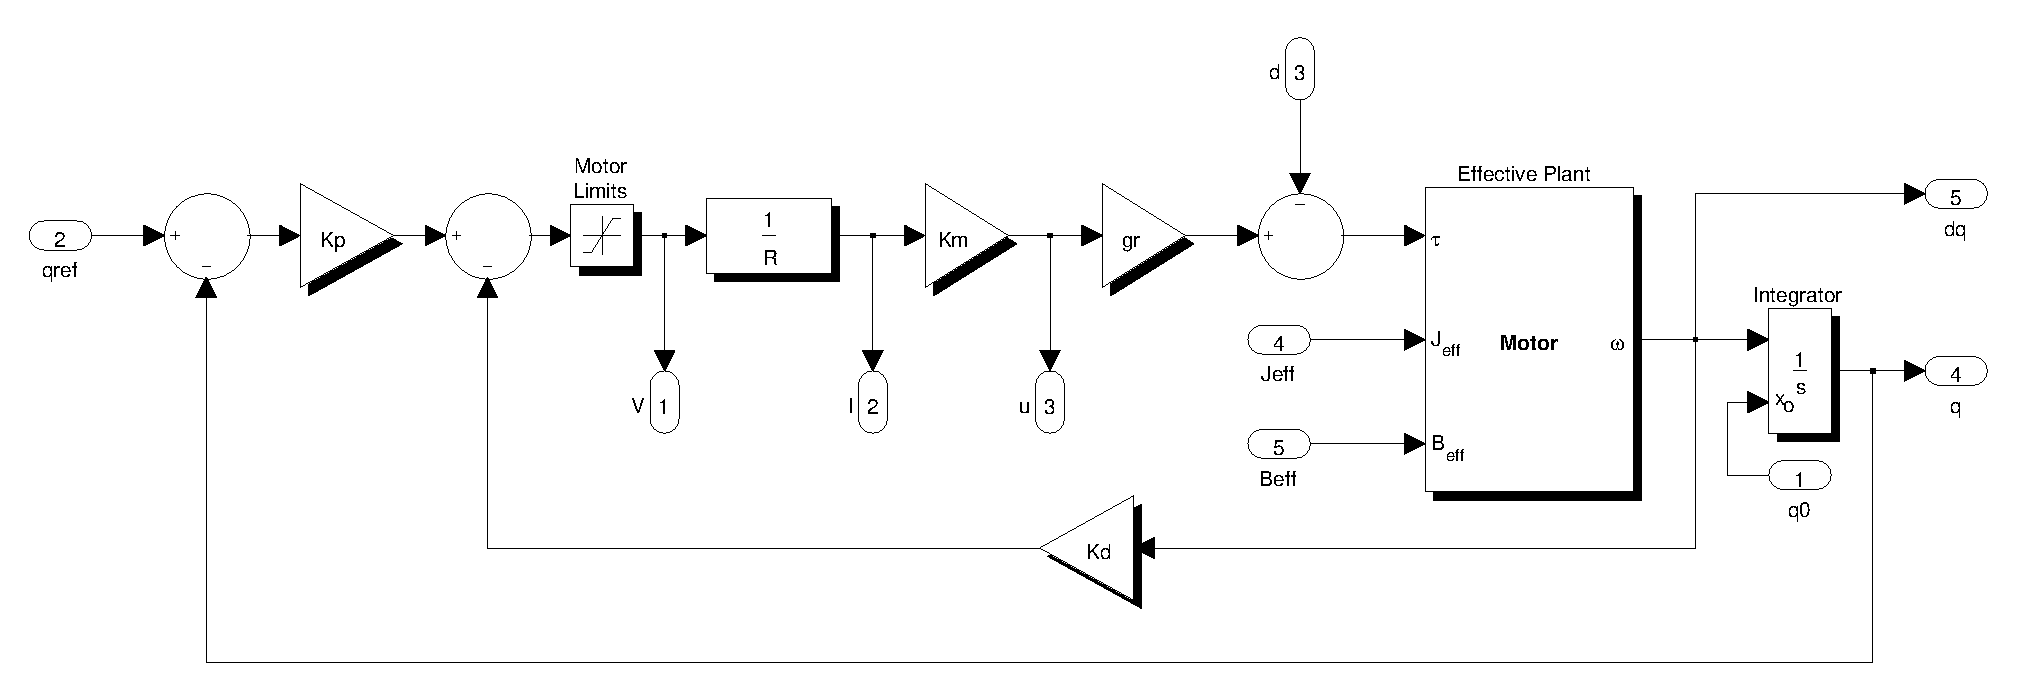
\includegraphics[scale=0.5]{fig/experiments/pdmotorcontroller.eps} 
  	\caption{PD controller model for independent joint control with actuator dynamics.}
	\label{fig:pdmotorcontroller}
\end{figure}

To improve the estimate of the motor side inertia, $a_{kk}$ is required in (\ref{eq:actdyn6}). The dynamic simulation package used in Section~\ref{sec:simulations_and_results} is based on the Matlab/Simulink environment and uses the SimMechanics toolbox which does not allow the mass matrix $\inertia$ to be isolated. Algorithm~\ref{alg:massdiag} was used to compute the mass matrix and extract the diagonal terms at each time step. \\

\begin{algorithm}[H]
 \SetAlgoLined
 Initialization\;
 Set $\vec{q} = \vec{q}_0$, $\vec{\dot q} = \vec{\dot q}_0$, $\vec{\ddot q} = \vec{0}$\;
 \While{1}{
  Compute $\hat{\vtau}$ using RNE with $\vec{\ddot q} = \vec{0}$\;
  \For{$i = 1$ to $n$}{
  Set $\tilde{\vec{g}} = \vec{0}$, $\mathbf{\tilde{\dot{q}}} = \vec{0}$, $\mathbf{\tilde{\ddot{q_i}}} = 1$, $\mathbf{\tilde{\ddot{q_j}}} = 0$ $[j \ne i]$\;
  Compute $\tilde{\vtau}$ using RNE\;
  Form $i$-th column: $\inertia_{i} = \tilde{\vtau} - \hat{\vtau}$
  }
  Combine columns to form $\inertia$\;
  Select diagonal elements of $\inertia$\;
 }
 \caption{Computing mass matrix diagonal terms with RNE algorithm}
 \label{alg:massdiag}
\end{algorithm}

% section actuator_model (end)

\section{HIL Architecture} % (fold)
\label{sec:hil_architecture}
The architecture used to control the physical 14 DOF bipedal robot is presented in this section. In general, controlling DC motors requires a controller (to host the control algorithm) and a driver (typically serves as a power amplifier). The controller outputs a low voltage control signal which is amplified by the driver and applied to the terminals of the motor. Encoders are used to sense the rotor position used by the controller for closed loop control. 

The physical bipedal robot in Section~\ref{sub:mechanical_implementation} is treated as the plant. Using Quanser's QUARC toolbox, control algorithms developed in the Simulink environment can be compiled for a variety of target platforms ranging from embedded microcontrollers to standard PC. This allows the use of a shared codebase for simulation and for the physical hardware. The control algorithms used for the biped are compiled and executed on a PC which communicates with the physical hardware through a data acquisition (DAQ) board. A separate and dedicated voltage amplifier is used to drive the DC motors from a low voltage analog control signal (labeled ``amplifier command'' on Figure~\ref{fig:hilarch}) from the controller via the DAQ. As an interim solution, Quanser provided the author with a Q8-USB (DAQ board) and a VoltPAQ (voltage amplifier) shown in Figure~\ref{fig:bipedwired}.

\begin{figure}[!h]
	\centering
    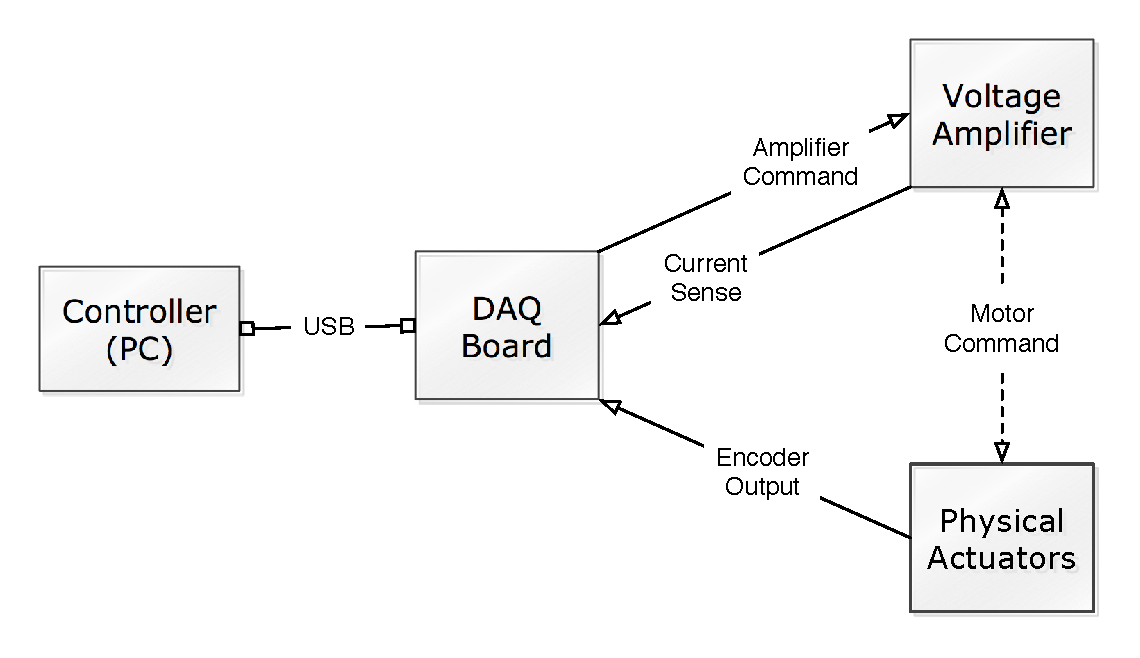
\includegraphics[scale=0.65]{fig/experiments/hilarchitecture.eps} 
  	\caption{Hardware architecture used to control the physical bipedal robot leg.}
	\label{fig:hilarch}
\end{figure}

The actuator subassemblies selected in Section~\ref{sub:final_configurations} were preassembled with incremental optical encoders mounted to the motor side. These encoders output digital signals on two channels.  These digital signals are passed back to the controller running on the PC via the DAQ. Using quadrature decoding, the motor angle $\Theta _m$ can be retrieved from the encoder output in degrees: 

\begin{equation}
	{\Theta _m} = \frac{{360}}{{n \cdot l}} \cdot Encoder_{output}
\end{equation}

Where $n = 4$ for quadrature (4X) decoding and $l$ is the lines per revolution specified from the encoder manufacturer. Using the relationship between the motor variables and the joint variables in (\ref{eq:actdyn2}), an estimate of the $k$-th link side angle (at the output of the gearhead) can be obtained: 

\begin{equation}
	{q_k} = \frac{{360}}{{4 \cdot l \cdot {g_{{r_k}}}}} \cdot Encode{r_k}
	\label{eq:quadrature}
\end{equation}

This is only an estimate of the joint angle since there are drivetrain losses (i.e. in the gearhead) which are ignored by an encoder mounted to the motor side. 

\subsection{Parallel Models} % (fold)
\label{sub:parallel_models}

The ability to develop a single controller and target either a simulation environment or the physical hardware is extremely useful. Using the Quanser's QUARC toolbox, a Q8-USB (DAQ) board and a VoltPAQ (voltage amplifier), the control algorithms were redeveloped as parallel models capable of switching target platforms (shown in Figure~\ref{fig:parallelmodels}).

\begin{figure}[!h]
	\centering
    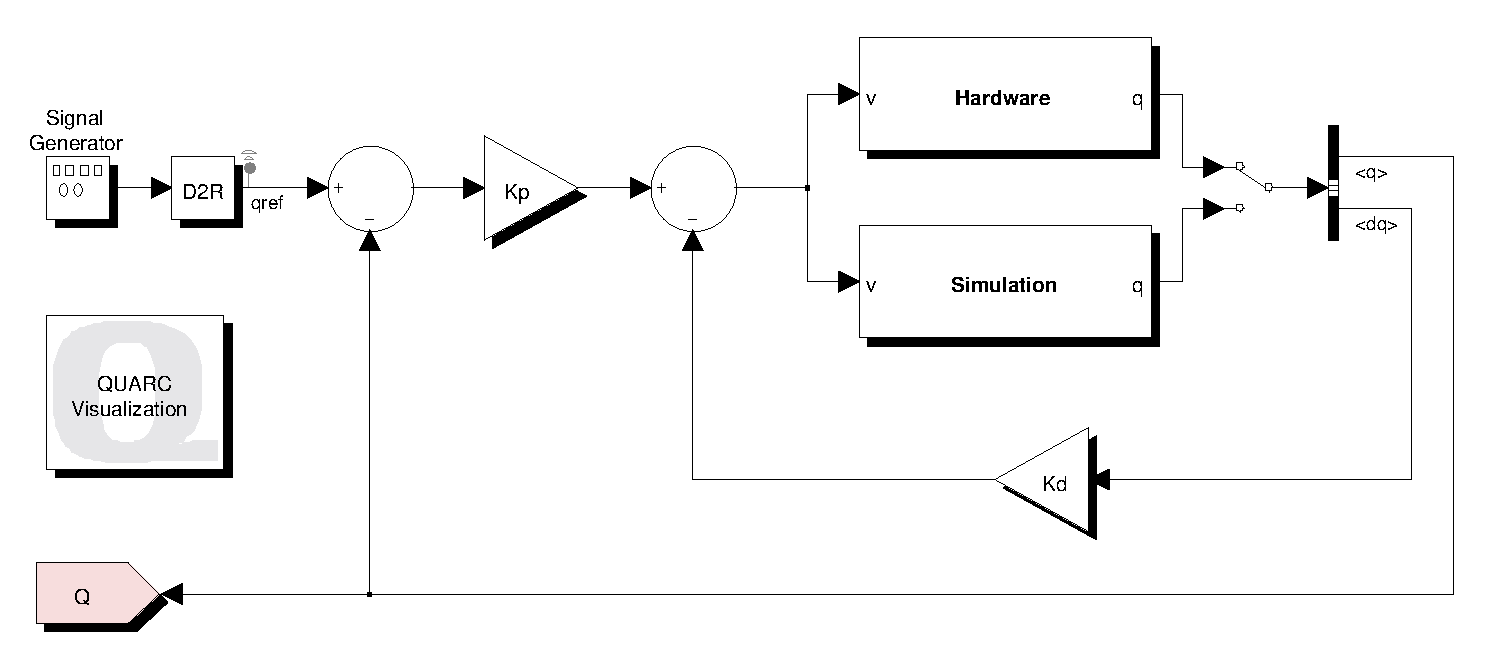
\includegraphics[scale=0.6]{fig/experiments/parallelmodels.eps} 
  	\caption{Parallel models designed to target either simulations or physical hardware with the same controller.}
	\label{fig:parallelmodels}
\end{figure}

In the physical environment mode shown in Figure~\ref{fig:hilmodel}, the hardware target subsystem is initialized to interface with the Q8-USB DAQ board. The control algorithm running on the PC communicates with the physical hardware using ``HIL Read'' and ``HIL Write'' blocks which communicate with the DAQ over USB. The PD controller output is an analog signal corresponding to the desired voltage at the motor terminals (amplifier command). The DAQ also reads the raw digital signals from the motor side encoders. The VoltPAQ voltage amplifier also provides the ability to read the current in the armature circuit ($i_a$) of the DC motor. This value is passed back to the controller through the DAQ using an analog channel. Due to the noise in the current sensor, a low pass filter is needed. The quadrature decoding formula (\ref{eq:quadrature}) is used to obtain the joint angle for the closed loop feedback. The link side angle information is also used to determine whether a joint is out of its limits. The controller detects and sends a ``shut down'' command to the amplifier channel if it is. 

\begin{figure}[!h]
	\centering
    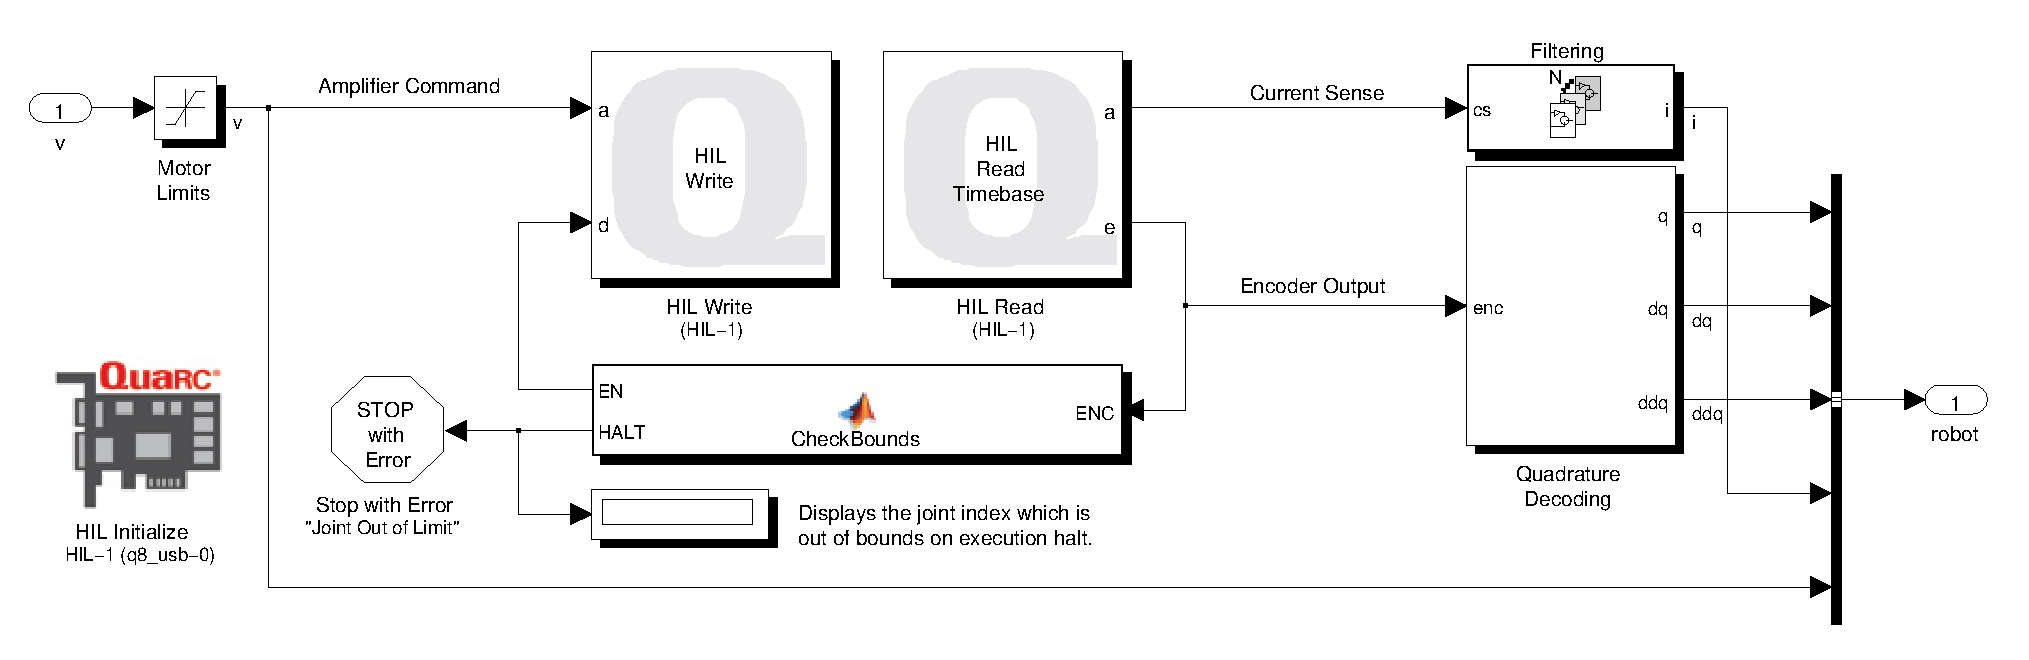
\includegraphics[scale=0.5]{fig/experiments/hilmodel.eps} 
  	\caption{HIL subsystem from Figure~\ref{fig:parallelmodels} used to target physical hardware with voltage control signal.}
	\label{fig:hilmodel}
\end{figure}

In the simulated environment mode, the controllers were reformulated to use the voltage signal as the control input. The simulation target subsystem shown in Figure~\ref{fig:simmodel} models the actuator dynamics and treats the link side torques as a disturbance input. The VoltPAQ amplifier gain ($3$ V/V) is applied to the voltage control signal to model the effective voltage at the motor terminals. The actuator dynamics are simulated with the motor ($R$, $K_m$, $K_b$, $J_m$ and $B_m$) and gearhead ($g_r$) parameters. The link side variables are obtained by applying the gear ratio to the motor velocity $\dot{\Theta}_m$ to obtain $\dot{q}$. The joint positions and accelerations are computed by taking the integral and derivative of $\dot{q}$, respectively. The joint angles, velocities and accelerations ($q$, $\dot{q}$, $\dot{\dot{q}}$) are used with inverse dynamics to compute the effective link side torques, which is fed back as a disturbance input to the simulated motor model. 

\begin{figure}[!h]
	\centering
    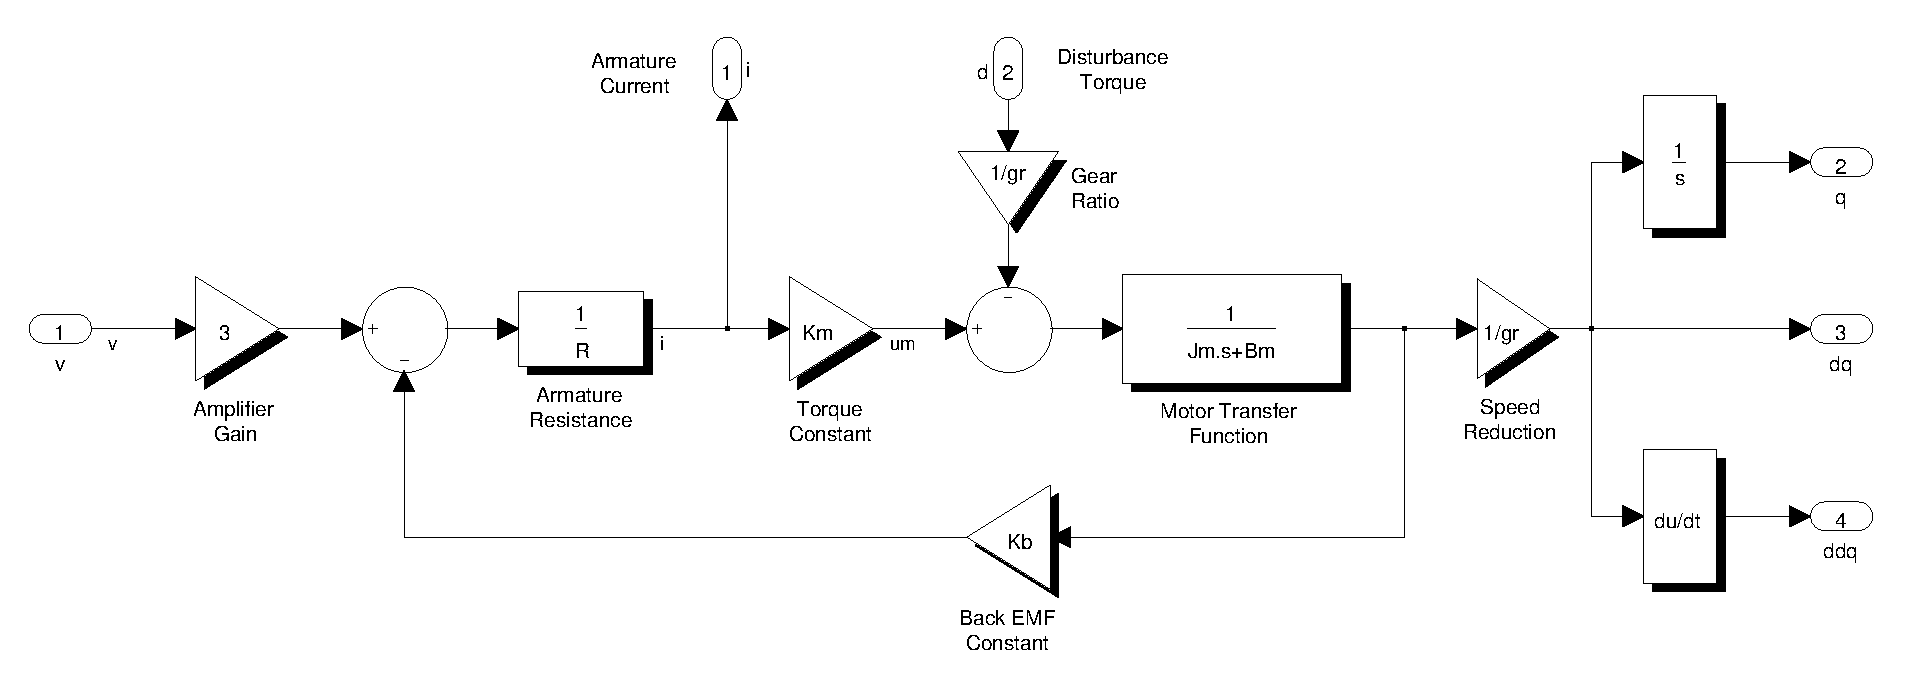
\includegraphics[scale=0.5]{fig/experiments/simmodel.eps} 
  	\caption{Subsystem from Figure~\ref{fig:parallelmodels} used to target the simulated environment with voltage control signal.}
	\label{fig:simmodel}
\end{figure}

Note that the full dynamic model of the 7 DOF leg is used for the plant in the simulation part of the experiments. The simplified dynamics are only used by the controller. 

% subsection parallel_models (end)

% section hil_architecture (end)

\section{Single DOF Validation} % (fold)
\label{sec:1dof_validation}
This section describes the experiments validating the simulation models for single DOF controllers using the HIL environment. Parallel models developed in Section~\ref{sub:parallel_models} were used to compare the results from simulation to the physical hardware. 

\subsection{Joint Tracking} % (fold)
\label{sub:joint_tracking}
Local PD controllers are used to track the joint level trajectories. The parallel model shown in Figure~\ref{fig:parallelmodels} was developed to tune the proportional ($K_P$) and derivative ($K_D$) gains for individual joints on the bipedal robot. First, the gains were tuned in the simulation environment to achieve the desired tracking performance. The shared controller architecture was then switched to target the physical hardware to validate the tracking results. 

The experimental results presented in this section compare the tracking performance of three joints in simulation and in hardware. Each joint tracks a sinusoidal reference trajectory at $0.5 Hz$. The amplitude and bias of each reference trajectory is selected to maintain the motion within the joint limits. Figures~\ref{fig:hipyawtracking}, \ref{fig:hippitchtracking} and \ref{fig:kneepitchtracking} compare the tracking performance for the hip yaw, hip pitch and knee pitch joints, respectively. 

\begin{figure}[!h]
	\begin{center}
	\subfigure{\includegraphics[scale=0.45]{fig/experiments/hipyawtrackingsim.eps}}
	\subfigure{\includegraphics[scale=0.45]{fig/experiments/hipyawtrackinghil.eps}}
	\end{center}
  	\caption{Hip yaw joint tracking results for simulation and hardware.}
	\label{fig:hipyawtracking}
\end{figure} 

% \begin{figure}[!h]
% 	\begin{center}
% 	\subfigure{\includegraphics[scale=0.45]{fig/experiments/hipyawvoltages.eps}}
% 	\subfigure{\includegraphics[scale=0.45]{fig/experiments/hipyawcurrents.eps}}
% 	\end{center}
%   	\caption{Hip yaw joint voltage and current in simulation and hardware.}
% 	\label{fig:hipyawelectrical}
% \end{figure} 

\begin{figure}[!h]
	\begin{center}
	\subfigure{\includegraphics[scale=0.45]{fig/experiments/hippitchtrackingsim.eps}}
	\subfigure{\includegraphics[scale=0.45]{fig/experiments/hippitchtrackinghil.eps}}
	\end{center}
  	\caption{Hip pitch joint tracking results for simulation and hardware.}
	\label{fig:hippitchtracking}
\end{figure} 

% \begin{figure}[!h]
% 	\begin{center}
% 	\subfigure{\includegraphics[scale=0.45]{fig/experiments/hippitchvoltages.eps}}
% 	\subfigure{\includegraphics[scale=0.45]{fig/experiments/hippitchcurrents.eps}}
% 	\end{center}
%   	\caption{Hip pitch joint voltage and current in simulation and hardware.}
% 	\label{fig:hippitchelectrical}
% \end{figure} 

\begin{figure}[!h]
	\begin{center}
	\subfigure{\includegraphics[scale=0.45]{fig/experiments/kneepitchtrackingsim.eps}}
	\subfigure{\includegraphics[scale=0.45]{fig/experiments/kneepitchtrackinghil.eps}}
	\end{center}
  	\caption{Knee pitch joint tracking results for simulation and hardware.}
	\label{fig:kneepitchtracking}
\end{figure} 

% \begin{figure}[!h]
% 	\begin{center}
% 	\subfigure{\includegraphics[scale=0.45]{fig/experiments/kneepitchvoltages.eps}}
% 	\subfigure{\includegraphics[scale=0.45]{fig/experiments/kneepitchcurrents.eps}}
% 	\end{center}
%   	\caption{Knee pitch joint voltage and current in simulation and hardware.}
% 	\label{fig:kneepitchelectrical}
% \end{figure} 
 
% subsection joint_tracking (end)

With the tuned PD gains, the tracking performance on the physical hardware is nearly identical to the simulation environment. Hip yaw joint tracking (Figure~\ref{fig:hipyawtracking}) shows that there is a very small but negligible lag on the physical hardware when compared to the simulated system. Hip pitch joint tracking (Figure~\ref{fig:hippitchtracking}) shows perfect tracking for the simulated system while there are small disturbances near the peaks of the sinusoidal wave on the physical hardware. This discrepancy is due to the backlash problem discussed in Section~\ref{sub:mechanical_implementation}. The simulated system demonstrates perfect tracking since backlash is not modeled. However, the PD controller gains are sufficiently high for the physical system to overcome the disturbances due to backlash and achieve near perfect tracking. 

% When the hip joint motion changes direction (i.e. at the peaks of the wave) on the physical system, the backlash in the knee   

% section 1dof_results (end)

\section{Motion Control Validation} % (fold)
\label{sec:motion_control_validation}
This section describes the experiments validating the motion control framework in Section~\ref{sub:control_strategy} using the HIL environment. The parallel model concept was extended to develop higher level task space controllers to generate the joint level trajectories for simulation and hardware. The interim control electronics provided by Quanser Inc are limited to controlling 7 DOF simultaneously. Therefore, only a single 7 DOF bipedal robot leg wired to the control electronics was used for the experiments in this section. The biped's torso was rigidly attached to the supporting frame in the fixed configuration, removing the 6 unactuated DOF. The Jacobian matrix used to map the task space and joint space velocities in (\ref{eq:jmap}) is reduced to: 

\begin{eqnarray}
	\J{}{} &=& \begin{bmatrix} \partial \qact \\ \end{bmatrix}_{m \times n} \\
	\dqref &=& \J{}{\#} \dxref \label{eq:calcqref}
\end{eqnarray}

Where $n = 7$ is the actuated and controllable DOF supported by the control electronics. The joint level commands are generated from the task space trajectories ($\dxref$) using (\ref{eq:calcqref}). Alternatively, the prioritized task space control scheme in Section~\ref{sub:control_strategy} can be used to simultaneously satisfy high priority constraints. The mapping provided by (\ref{eq:priori}) is simplified by removing the actuator selection matrix $\mathbf{S}$, since there are no unactuated DOF. 

The fixed configuration of the supporting frame causes the 7 DOF leg to naturally hang straight at the start of each experiment (i.e. $\q = \mathbf{0_{7 \times 1}}$). This represents a singular configuration of the leg. In Section~\ref{sec:1dof_validation}, the joint level commands were provided directly to the local PD controller. Computing the joint level commands with (\ref{eq:calcqref}) requires inverting the Jacobian matrix, which is problematic for singular configurations. To address this issue, each experiment starts by directly controlling the joint level trajectories for $t_{init} = 5$ seconds to manually move the leg into a non-singular configuration. 

\subsection{Planar Motion Control} % (fold)
\label{sub:planar_motion_control}
Some motions during the bipedal gait cycle can be simplified to a planar motion control problem. Common motions during the swing phase include bending of the knee joint and tracking an arc-like trajectory for the swing foot position. For these cases, the 3 pitch joints in the 7 DOF leg are primarily used to carry out the desired motion. A simplified version of the motion control framework (\ref{eq:calcqref}) can be used to control the swing foot position in the biped's sagittal plane.

\begin{equation}
	\dqref = \J{}{\#} \dxswing
\end{equation}

\begin{figure}[!h]
	\centering
    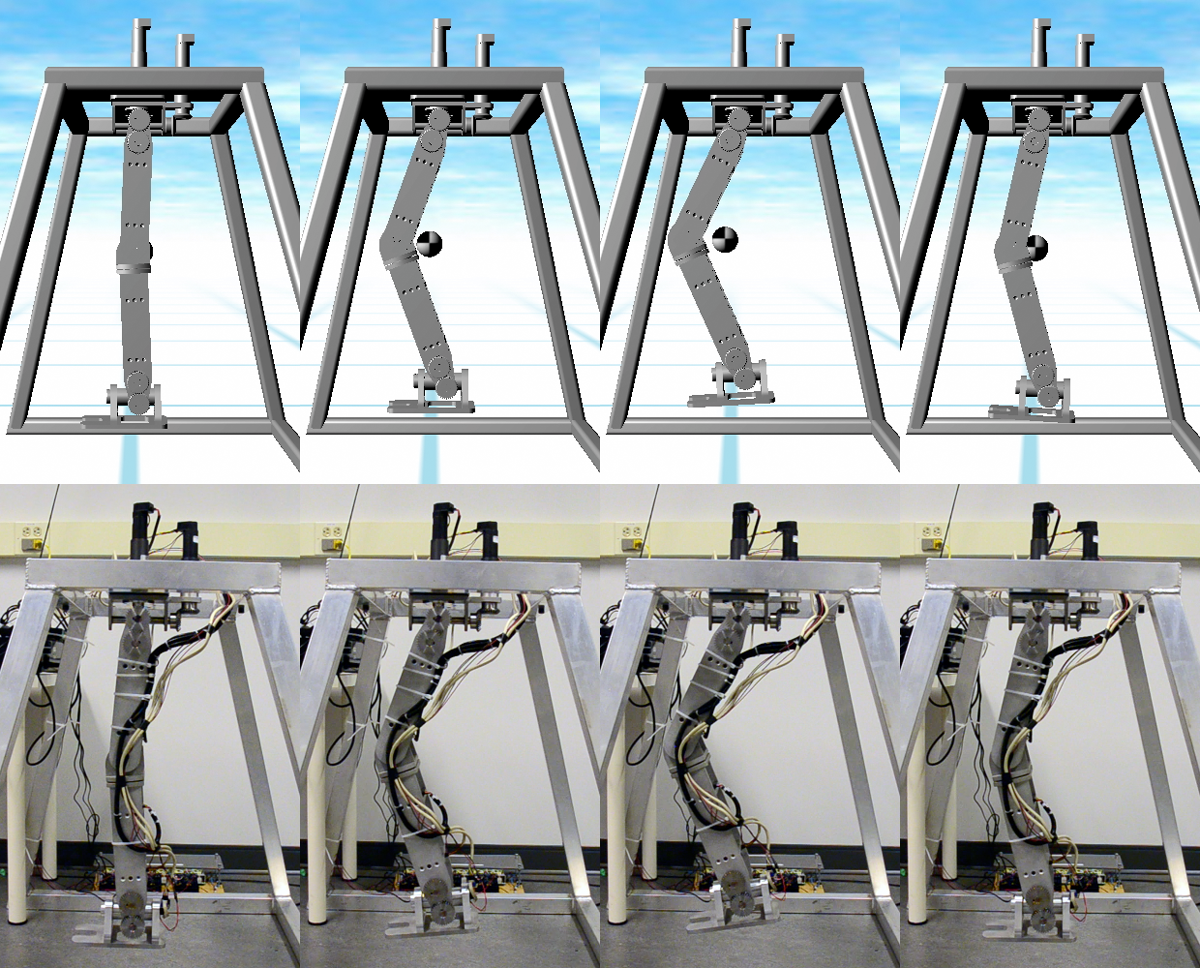
\includegraphics[scale=0.37]{fig/experiments/kneebendframes.png} 
  	\caption{Captured frames while raising the foot in simulation and physical hardware.}
	\label{fig:kneebendframes}
\end{figure}

\subsubsection{Raising the Foot} % (fold)
\label{ssub:knee_bending_motion}

In this experiment, the foot position is raised vertically, resulting in a knee bending motion. The frame captures shown in Figure~\ref{fig:kneebendframes} demonstrate this experiment in simulation and on the physical hardware. The first frame in the sequence is the home configuration of the 7 DOF leg at start of each experiment (i.e. at $t = 0$). The second frame represents a slightly angled configuration of the leg joints after $t_{init} = 5$ seconds. The remaining frames demonstrate the foot raising motion for this experiment. 

\begin{figure}[!t]
	\begin{center}
	\subfigure{\includegraphics[scale=0.45]{fig/experiments/simkneebendp.eps}}
	\subfigure{\includegraphics[scale=0.45]{fig/experiments/hilkneebendp.eps}}
	\end{center}
  	\caption{Task space trajectory tracking for bending the knee and raising the leg in simulation and hardware.}
	\label{fig:kneebendp}
\end{figure} 

PD control was also applied on the task space level to improve performance of the motion controller. The gains were tuned in simulation to achieve the desired tracking performance before attempting the experiment on the physical hardware. The foot position tracking using $K_P = 10$ and $K_D = 0.1$ is shown in Figure~\ref{fig:kneebendp} in simulation and on hardware. The experimental  results demonstrate the simplified version of the motion control framework with $n = 3$ DOF. The pitch joint trajectories are automatically generated from the desired swing foot height and the resulting motion bends the knee joint as the foot is raised. The joint level trajectories were tracked by the local PD controllers with individual gains tuned from Section~\ref{sec:1dof_validation}. 

% subsubsection knee_bending_motion (end)

\subsubsection{Swing Foot Motion} % (fold)
\label{ssub:swing_foot_motion}

In this experiment, the foot is commanded to track an arc-like trajectory while forward progress is made along the plane. The resulting motion is commonly used during the swing phase of the gait cycle for a bipedal robot to take a step. The frame captures shown in Figure~\ref{fig:swingmotionframes} demonstrate this motion in simulation and on hardware. The task space control gains tuned in the previous section were reused for this experiment. 

\begin{figure}[!t]
	\centering
    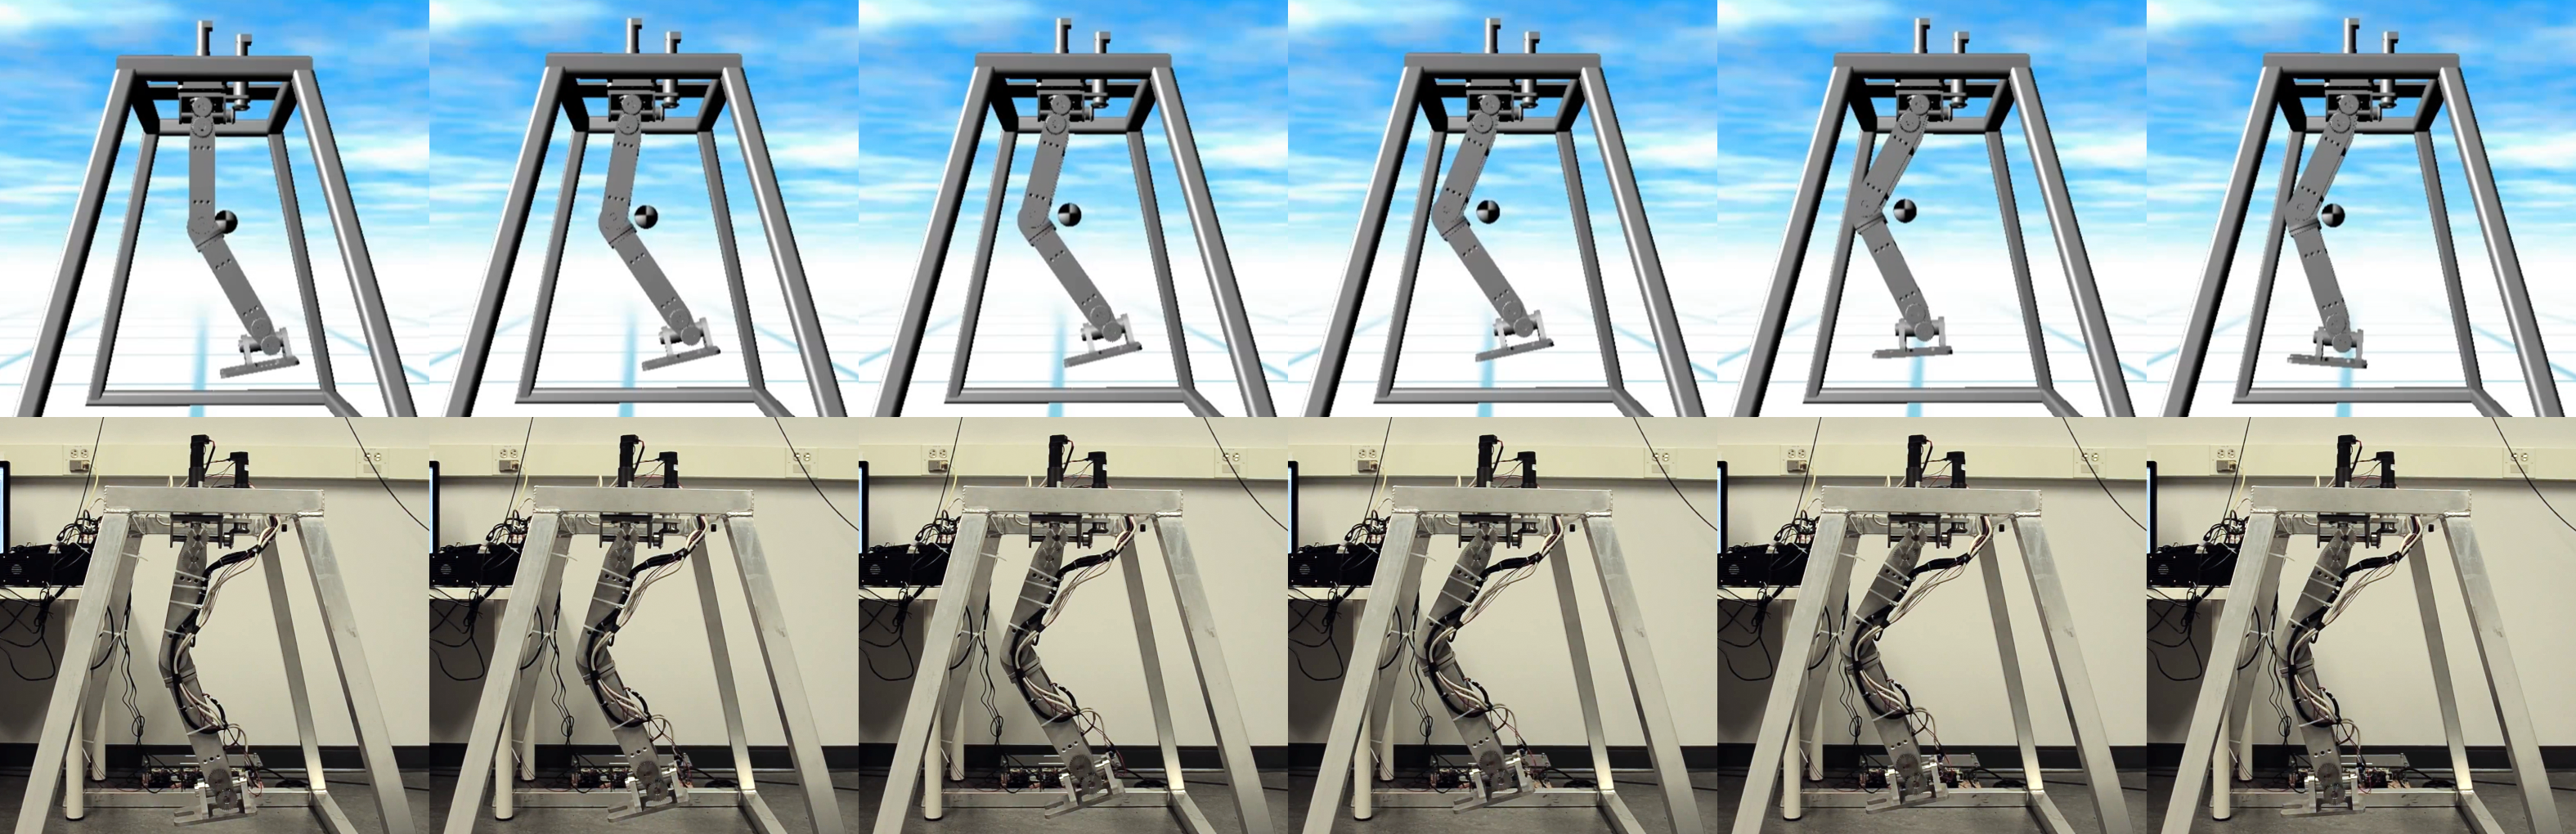
\includegraphics[scale=0.38]{fig/experiments/swingmotionframes.png} 
  	\caption{Captured frames during swing foot motion experiment in simulation and physical hardware.}
	\label{fig:swingmotionframes}
\end{figure}

\begin{figure}[!b]
	\begin{center}
	\subfigure{\includegraphics[scale=0.45]{fig/experiments/simswingfootp.eps}}
	\subfigure{\includegraphics[scale=0.45]{fig/experiments/hilswingfootp.eps}}
	\end{center}
  	\caption{Task space trajectory tracking for swing foot motion in simulation and hardware.}
	\label{fig:swingfootp}
\end{figure} 

The task space tracking results for the swing foot motion is shown in Figure~\ref{fig:swingfootp}. Similar to the previous planar motion experiment, the hardware closely matches the simulated system with the tuned gain parameters. The swing foot trajectory on the physical hardware along the $x$ direction is not as smooth as its simulated counterpart. Unmodeled backlash in the pitch joints (i.e. the knee) is the cause behind this difference. However, the PD control gains in the task space and joint space controllers are high enough to achieve the desired tracking performance. 

\begin{figure}[!t]
	\begin{center}
	\subfigure{\includegraphics[scale=0.45]{fig/experiments/simswingfootq.eps}}
	\subfigure{\includegraphics[scale=0.45]{fig/experiments/hilswingfootq.eps}}
	\end{center}
  	\caption{Joint space tracking of generated trajectories from higher level control during swing foot motion.}
	\label{fig:swingfootq}
\end{figure} 

The joint space tracking of the command signal generated by the motion control framework is shown in Figure~\ref{fig:swingfootq}.

% subsubsection swing_foot_motion (end)
\cleardoublepage
% subsection planar_motion_control (end)

\subsection{Whole Body Motion Control} % (fold)
\label{sub:whole_body_motion_control}
Most common motions for a 3D bipedal robot are not restricted to the planar case. These require control over the whole body during the gait cycle. The strategy developed in Section~\ref{sub:control_strategy} relies heavily on controlling the biped's motion through the Jacobian for the COM ($\J{COM}{}$) and both feet ($\J{STAND}{}$, $\J{SWING}{}$). These are used in conjunction with the prioritized control scheme to maintain stability in the off sagittal plane and generate a forward momentum for balance recovery with the 3D FPE approach. The 7 DOF experimental platform is labeled as the swing leg for the following experiments.  

\subsubsection{Circling COM Motion} % (fold)
\label{ssub:com_circular_motion}

\begin{figure}[!b]
	\centering
    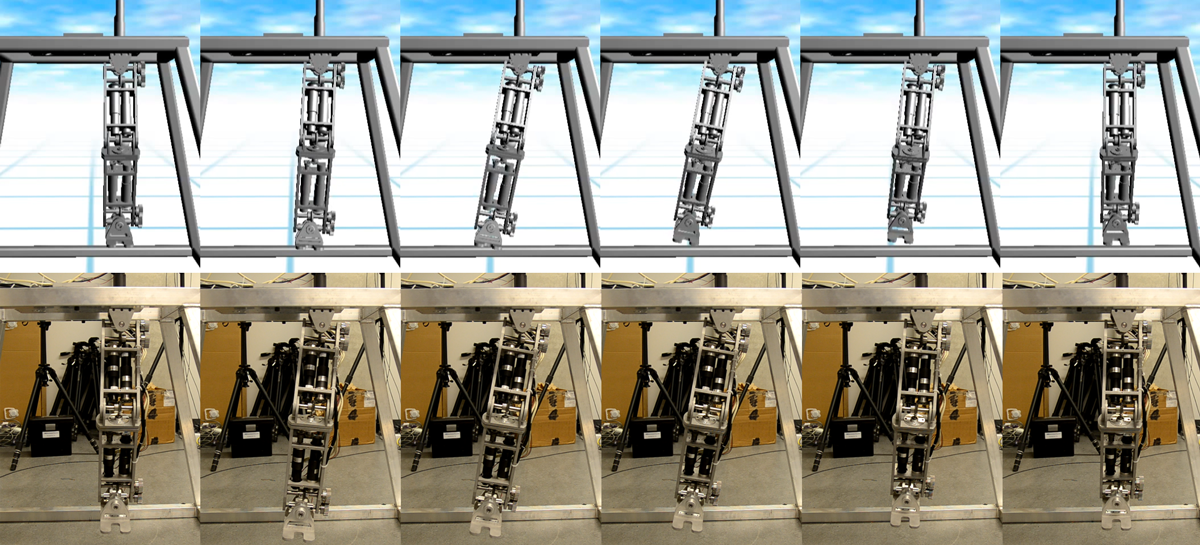
\includegraphics[scale=0.39]{fig/experiments/comcircleframes.png} 
  	\caption{Captured frames during COM circular experiment in simulation and physical hardware.}
	\label{fig:comcircleframes}
\end{figure}

A circular trajectory is generated for $\xcom$ on the $xy$-plane at a fixed height $z = h_{fixed}$. The height of the COM position at the end of $t_{init}$ is selected as this fixed height. Similarly to the planar case, the joint level commands are generated by the Jacobian mapping in (\ref{eq:jcomcirc}). 

\begin{equation}
	\dqref = \J{COM}{\#} \dxcom
	\label{eq:jcomcirc}
\end{equation}

$\dxcom$ represents the cartesian position of the foot in the world frame. The tracking results of the $\xcom$ following the circular trajectory are shown in Figure~\ref{fig:comcirctracking}. The initial task space control gains used in Section~\ref{sub:planar_motion_control} required retuning. The tuned gain values $K_P = 14$ and $K_D = 0.5$ achieved nearly identical performance on hardware and software. 

\begin{figure}[!h]
	\begin{center}
	\subfigure{\includegraphics[scale=0.45]{fig/experiments/simcomcirctracking.eps}}
	\subfigure{\includegraphics[scale=0.45]{fig/experiments/hilcomcirctracking.eps}}
	\end{center}
  	\caption{Task space tracking of circular COM motion in software and hardware.}
	\label{fig:comcirctracking}
\end{figure} 

% subsubsection com_circular_motion (end)

\subsubsection{Prioritized Motion} % (fold)
\label{ssub:prioritized_motion}

\begin{figure}[!h]
	\centering
    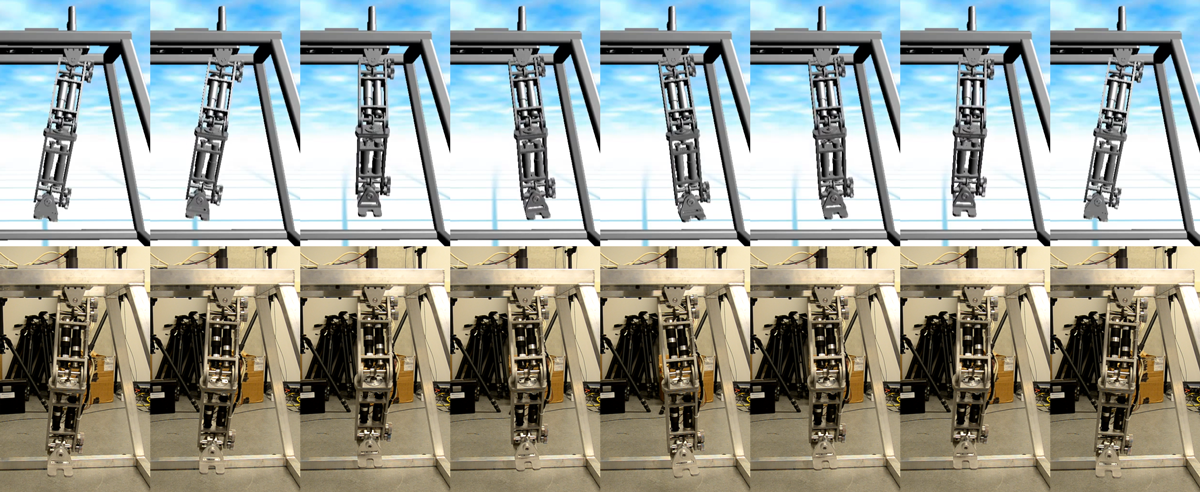
\includegraphics[scale=0.38]{fig/experiments/prioritizedframes.png} 
  	\caption{Captured frames during prioritized motion experiment in simulation and physical hardware.}
	\label{fig:prioritizedframes}
\end{figure}

The prioritized control scheme is used to project a low priority task ($\J{L}{}$, $\dxl$) onto the null space of a higher priority task ($\J{H}{}$, $\dxh$). This approach was used in Section~\ref{sub:control_strategy} to maintain the $\xcom$ position at the center of the support foot ($\xstand$) while the swing foot is lifted from the ground. A side stepping motion is generated for $\xswing$ to follow an arc-like trajectory along the biped's frontal ($yz$) plane as the high priority task for this experiment. The low priority task is selected to constrain the $\xcom$ motion parallel to the frontal plane. That is, $\xcom_x$ remains constant while ($\xcom_y, \xcom_z$) move freely during the side stepping motion. Frame captures taken during this experiment are shown in Figure~\ref{fig:prioritizedframes}. The joint level commands  consistent with the prioritization in (\ref{eq:taskprioritization}) are computed using (\ref{eq:priori}).

\begin{IEEEeqnarray}{rClrCl}
	\J{H}{} & = &
	\begin{bmatrix}
		\J{SWING}{}
	\end{bmatrix} &
	\dxh & = &
	\begin{bmatrix}
		\dxswing
	\end{bmatrix} \nonumber \\
	\J{L}{} & = &
	\begin{bmatrix}
		\J{COM}{}_x
	\end{bmatrix}  &
	\dxl & = &
	\begin{bmatrix}
		\dot{\mathbf{x}}_{\textbf{COM}x}
	\end{bmatrix} \nonumber \\
	\label{eq:taskprioritization}
\end{IEEEeqnarray}

$\J{COM}{}_x$ and $\dot{\mathbf{x}}_{\textbf{COM}x}$ represent the $x$-component (i.e. the first row) of the COM Jacobian and task space error $\Delta \xcom$. The prioritized tracking results for this experiment are shown in Figure~\ref{fig:prioritizedtracking}. The tracking performance of the high priority tasks are almost identical in both cases. However, the low priority tracking performance is noisier on the hardware when compared to the simulation results. 

\begin{figure}[!t]
	\begin{center}
	\subfigure{\includegraphics[scale=0.45]{fig/experiments/simprioritizedtracking.eps}}
	\subfigure{\includegraphics[scale=0.45]{fig/experiments/hilprioritizedtracking.eps}}
	\end{center}
  	\caption{Tracking high and low priority task space trajectories in simulation and hardware.}
	\label{fig:prioritizedtracking}
\end{figure} 

% subsubsection prioritized_motion (end)

% subsection whole_body_motion_control (end)

% section motion_control_results (end)

\section{Summary} % (fold)
\label{sec:experiments_summary}
Validating control algorithms on physical hardware is important due to modeling imperfections in the simulation environment. The physical 14 DOF bipedal robot developed in earlier chapters was used for experimental validation. The custom control electronics solution was developed by Quanser Inc for the bipedal robot. Unfortunately, the complete solution was not ready in time for experimental validation. An interim solution was used to control an assembled 7 DOF leg for experimental validation in this section. 

For the physical hardware, DC motors are controlled by a voltage signal $v_m$. A second order system was used to model the actuator dynamics and reformulate the existing controllers which controlled the link side torques $\tau _k$. Independent joint control decouples each joint for individual control. Since this approach does not account for the coupled dynamics of the overall system, the link side torques are treated as a disturbance to the actuator dynamics model. The effective motor inertia is reformulated to include the link inertia seen by the joint. A generic RNE-based algorithm was used to extract the mass matrix of the system at every time step to compute the effective motor inertia.

The HIL architecture was developed using Quanser's QUARC toolbox, DAQ board and a voltage amplifier. The controller code developed in Simulink was targetted to execute on the PC. The DAQ board allowed the PC-based controller to communicate with the physical hardware through analog and digital I/O. Quadrature decoding was on the encoder output to obtain the link side joint angles on physical hardware for closed loop feedback control. Parallel simulation models were developed for experimental validation to target the physical hardware or the simulated actuator dynamics. 

The parallel models were used to demonstrate key components of the control approach developed in this thesis on physical hardware. Single DOF validation was used to individually tune the PD controller gains at the joint level. Once the desired tracking performance was achieved, the task space motion control framework used to generate the joint level commands was validated. Starting with a simple planar motion control problem, the foot position was controlled in the task space to achieve knee bending and an arc-like swing foot motion. Joint level command signals were generated for the local PD controllers using the simplified motion control framework. PD control was also applied at the task space level to improve tracking performance of the motion controller. Finally, the complete motion control framework was demonstrated in simulation and on the physical hardware through the COM tracking experiment. By using all (7) actuated DOF in the leg, the controller was able to sufficiently track a task space trajectory for the COM position. The prioritized task space control scheme was also demonstrated by restricting the $\xcom$ motion to a plane in the null space of the higher priority constraint of tracking an arc-like trajectory for side-to-side stepping. 

% section discussion (end)

% chapter experiments (end)